\chapter{WebSocket}
\label{chapter:websocket}

This chapter provides a historical background of the real-time web and an introduction to the WebSocket API and the WebSocket protocol. Furthermore, the design philosophy and use cases of WebSocket are studied and an overview of related technologies is given.

\section{The Real-Time Web}

The web has gone through tremendous changes since the original \textit{Proposal for a HyperText Project} by Tim Berners-Lee and Robert Cailliau was published in 1990. The authors of the proposal envisioned an information system consisting of nodes in a network. These nodes would contain information of various kinds that a user could browse \cite{berners1990worldwideweb}. The web was initially intended for static content so the first version of HTTP was optimized for synchronous request-response communication \cite{berners1991original}. The emergence of client-side scripting languages, in the mid-nineties, paved the way for web applications capable of asynchronous communication. JavaScript and the XMLHttpRequest API became the core components in a set of web development techniques, termed AJAX, that could be used to fetch and display content on websites without requiring a full page reload \cite{garrett2005ajax}.
\\ \\
The next major step in the development of web applications largely revolved around simulating server-push events to mimic real-time behavior. As HTTP uses a request-response paradigm (Figure~\ref{fig:request-response}) it is not a suitable protocol for applications with real-time functionality. Nevertheless, quite a few solutions to work around the limitations of HTTP were invented. The solutions can be used to provide functionality that end-users experience as real-time despite the half-duplex nature of HTTP. The first of the solution to emerge was polling (Figure~\ref{fig:polling}) followed by long-polling (Figure~\ref{fig:long-polling}) and streaming (Figure~\ref{fig:streaming}).

\begin{figure}[h!]
	\centering
	\subfigure[Request-response]{\label{fig:request-response}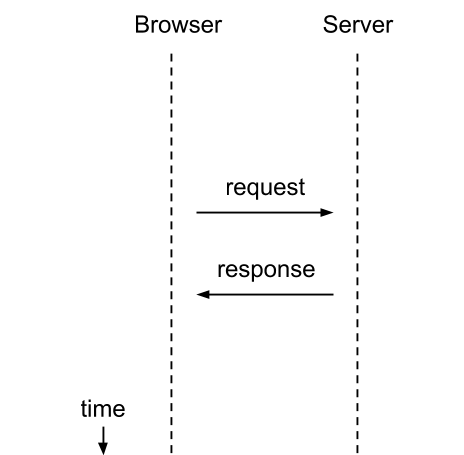
\includegraphics[width=0.45\textwidth]{images/request-response}} \hfill
	\subfigure[Polling]{\label{fig:polling}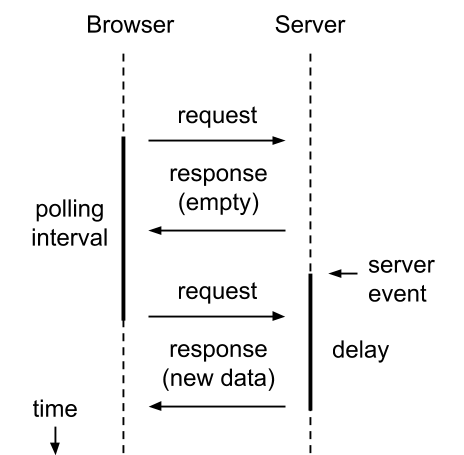
\includegraphics[width=0.45\textwidth]{images/polling}}
	\caption{Client-server communication}
\end{figure}

\subsection{Polling, Long-Polling and Streaming}

Polling is a technique used by clients to retrieve data from a server by making periodic requests for new information. The requests are made at a regular interval and the server responds to each request whether new data is available or not. This approach automates the process of requesting new data on the client-side and can be a good solution if the interval between the arrival of new data on the server-side is known \cite{pimentel2012communicating}. If the interval between data updates on the server-side in not know polling can lead to unnecessary requests, in case of a too short polling interval, or slow updates on the client-side, if the polling interval is too long. A HTTP requests includes between 500 and 800 bytes of protocol overhead which leads to ineffective data transfer for short messages and useless data transfer for empty responses \cite{grigorik2013high}. Polling is generally a bad solution for applications with unpredictable data updates, such as chat applications, because it can cause unnecessary data transfer and network load.
\\ \\
Long-polling is a techniques where a server responds to a hanging client request when new data is available. This techniques can lead to long-lived HTTP connections or timeouts if new data is not readily available moments after a client request. When a client either receives a response to a request or a timeout occurs it can open up a new hanging request for more data. Long-polling is an attempt to reduce the amount of unnecessary data transfer and network load caused by polling. This technique can work well for application with unpredictable data updates but in the case of high message volume or periodic data updates it does not provide performance improvement over polling \cite{grigorik2013high}. Long-polling is currently among the most widely used techniques for real-time data transfer on the web and is a popular fallback strategy for other real-time solutions \cite{modernizr}.
\\ \\
Streaming is similar to long-polling in the way that a client initiates a long-lived HTTP request that the server responds when new data is available. The main difference is that a server that has responded to a streaming request does not close the connections after it has responded. That can be a problem with regards to firewalls and web proxies that might buffer the responses which can lead to unreliable data transfer. Another problem is the lack of standardization as this technology is implemented differently across different browsers. This inconsistency makes streaming hard to implement into web applications that should provide the same functionality across different browsers. Streaming was supposed to address some of the issues with long-polling but did not manage to gain attraction because of its disharmony with the underlying infrastructure of the web and lack of standardization \cite{grigorik2013high}.

\begin{figure}[h!]
	\centering
	\subfigure[Long-polling]{\label{fig:long-polling}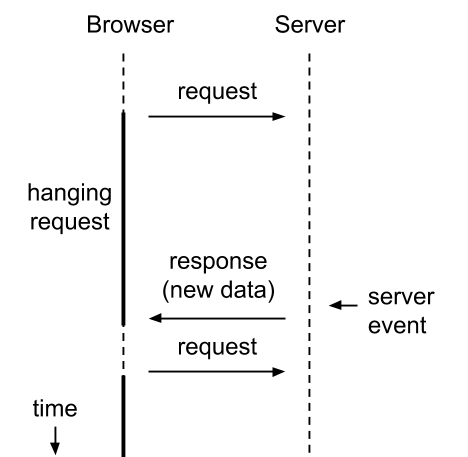
\includegraphics[width=0.45\textwidth]{images/long-polling}} \hfill
	\subfigure[Streaming]{\label{fig:streaming}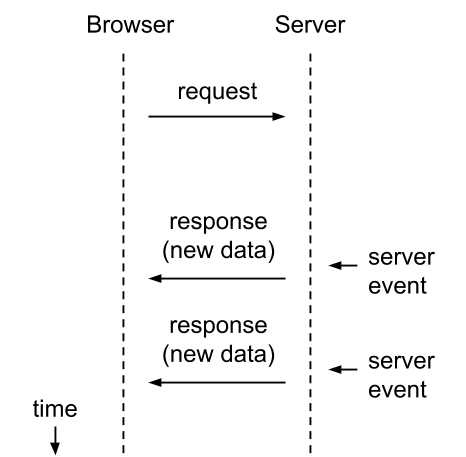
\includegraphics[width=0.45\textwidth]{images/streaming}}
	\caption{Client-server communication}
\end{figure}

\noindent
The underlying problem with the solutions presented before is that they are attempts to extend the functionality of HTTP to cover use cases it was not intended for. This requires various non-standardized workarounds which usually leads to increased complexity, reduced reliability and performance for applications. WebSocket was introduced, initially as a part of the HTML5 initiative, to provide a standardized foundation for real-time web applications to address those issues.

\section{WebSocket}

WebSocket is a standard for a full-duplex, bidirectional, single-socket connection over a single TCP connection. The WebSocket API is being standardized by the W3C and the WebSocket protocol has been standardized by the IETF as RFC 6455 \cite{hickson2011websocket,fette2011websocket}. The main goal of WebSocket is to provide a standardized, bidirectional communication mechanism for web applications. It is a thin layer on top of TCP that adds minor functionality to ensure compliance with the constraints of the web and existing HTTP infrastructure. WebSocket is not solely applicable to web applications and is intended to be extensible so future versions can be adjusted to be used any client and server application.

\begin{table}[h!]
\centering
\begin{tabular}{llll}
\hline
\textbf{Features}    & \textbf{TCP}        & \textbf{HTTP} & \textbf{WebSocket}       \\ \hline
Addressing           & IP address, port    & URL           & URL                      \\
Transmission         & Full-duplex         & Half-duplex   & Full-duplex              \\
Content              & Byte streams        & MIME			& Text, binary				 \\
Message boundaries   & No                  & Yes           & Yes                       \\
Connection oriented  & Yes                 & No            & Yes						  \\
\hline                         
\end{tabular}
\caption{Comparison of TCP, HTTP and WebSocket \cite{wang2013definitive}}
\label{table:tcpHttpWebsocketComparison}
\end{table}

\subsection{The WebSocket API}

The WebSocket API is an interface for the WebSocket protocol to initiate a bidirectional communication channel between a web application and a server \cite{hickson2011websocket}. A WebSocket connection is established through a HTTP request with an upgrade header. If the server supports the WebSocket protocol and accepts the update request the initial HTTP connection is replaced by a WebSocket connection on top of the same underlying TCP connection. The WebSocket constructor requires a URL argument (\url{ws://} or \url{wss://}) and has an optional protocol argument which lists the protocols supported by the application. After a connection has been established data can be transferred bidirectionally and asynchronously between the client and server. The communication requires considerably less protocol overhead than previous HTTP-based solutions for real-time data transfer. The API allows an application to listen to the \texttt{open}, \texttt{message}, \texttt{error} and \texttt{close} WebSocket events than can be used for callback functions. During the lifetime of a connection WebSocket objects have the \texttt{send()} and \texttt{close()} methods to transmit data and terminate the connection. In addition the \texttt{readySate}, \texttt{bufferedAmount} and \texttt{protocol} attributes can be used to provide more information about a WebSocket object. 

\subsection{The WebSocket Protocol}

The WebSocket protocol consists of an opening handshake, a data transfer phase and a closing handshake \cite{fette2011websocket}. The handshake starts with a HTTP request with a \texttt{Upgrade} field in the header where the client asks to upgrade the HTTP connection to the WebSocket protocol

\begin{figure}[h!]
\begin{verbatim}
GET wss://echo.websocket.org/?encoding=text HTTP/1.1
Host: echo.websocket.org
Connection: Upgrade
Upgrade: websocket
Origin: http://www.websocket.org
Sec-WebSocket-Version: 13
Sec-WebSocket-Key: soYsLdq15l8jOlybHiiHZg==
\end{verbatim}
\caption{Request headers of a WebSocket upgrade handshake}
\label{request-headers}
\end{figure}

\begin{figure}[h!]
\begin{verbatim}
HTTP/1.1 101 Web Socket Protocol Handshake
Connection: Upgrade
Date: Sun, 26 Apr 2015 11:34:08 GMT
Sec-WebSocket-Accept: qrKYhFFjmkJgSQCxW22hVJvUlHU=
Upgrade: websocket
\end{verbatim}
\caption{Response headers of a WebSocket upgrade handshake}
\label{response-headers}
\end{figure}

\noindent
The data transfer phase begins after a successful opening handshake. In the WebSocket protocol, data is transferred through a sequence of frames that are combined to form a logical application message. The WebSocket API is only concerned with messages while the WebSocket protocol takes care of splitting the messages into the frames, transporting them over a network, reassembling at the receivers end and finally notifies the receiver after a whole message has been received. A client sent WebSocket frame has 6 - 14 bytes of overhead and a server-sent one has 2 - 10 bytes. The different frame overhead size results from the payload length being represented in a variable length-field which allows small messages to use compact encoding while allowing the protocol to carry larger messages. Figure~\ref{protocol-framing} shows the WebSocket protocol framing.

\begin{figure}[h!]
\begin{verbatim}
 0                   1                   2                   3
 0 1 2 3 4 5 6 7 8 9 0 1 2 3 4 5 6 7 8 9 0 1 2 3 4 5 6 7 8 9 0 1
+-+-+-+-+-------+-+-------------+-------------------------------+
|F|R|R|R| opcode|M| Payload len |    Extended payload length    |
|I|S|S|S|  (4)  |A|     (7)     |             (16/64)           |
|N|V|V|V|       |S|             |   (if payload len==126/127)   |
| |1|2|3|       |K|             |                               |
+-+-+-+-+-------+-+-------------+ - - - - - - - - - - - - - - - +
|     Extended payload length continued, if payload len == 127  |
+ - - - - - - - - - - - - - - - +-------------------------------+
|                               | Masking-key, if MASK set to 1 |
+-------------------------------+-------------------------------+
| Masking-key (continued)       |          Payload Data         |
+-------------------------------- - - - - - - - - - - - - - - - +
:                     Payload Data continued ...                :
+ - - - - - - - - - - - - - - - - - - - - - - - - - - - - - - - +
|                     Payload Data continued ...                |
+---------------------------------------------------------------+
\end{verbatim}
\caption{The WebSocket protocol framing}
\label{protocol-framing}
\end{figure}

\noindent
The closing handshake is done to gracefully end the connection, with the knowledge of both sides of the communication, leading to the termination of the underlying TCP connection. There are several closing codes defined in the WebSocket protocol standard applicable for different scenarios.

\subsection{WebSocket Design Philosophy and Use Cases}

WebSocket is built as a small layer on top of TCP with minimal framing that can coexist with HTTP and deployed HTTP infrastructure. It is intended to be as close to raw TCP as possible given the constraints of the web. The eventual goal of WebSocket is to provide a simple and extensible protocol with support for higher-level protocols that facilitates the development of applications with real-time functionality.
\\ \\
The main use cases for WebSocket are web applications with real-time functionality that can be achieved through bidirectional communication between a client and a server. Typical examples would be chat applications, multiplayer games and news feeds to name a few. The extensibility and communication efficiency of WebSocket has also put the protocol into consideration for other use cases, such as in M2M communication \cite{perez2013electric,doukas2015providing}. For the future development of WebSocket technological trends, such as IoT, will most likely be taken into account. In case it manages to gain attraction the protocol has the potential to play an important role in future communication patterns.

\section{Related Technologies}

In addition to the HTTP-based solution and WebSocket there are more techniques that can be leveraged to build web applications with real-time functionality. Depending on the use case requirements, they can even be more suitable than WebSocket.

\subsection{Server-Sent Events}

Server-Sent Events is a standardized technology for servers to push text-based data to a client over a HTTP connection. Server-Sent Events is standardized by the W3C as a part of HTML5 \cite{hickson2009server}. The EventSource API and the event-stream protocol format of Server-Sent Events provide an efficient streaming implementation for text-based event data. This standard implementation abstracts away the underlying complexity of the server-to-client connection management and message parsing. Unlike WebSocket Server-Sent Event is transported over HTTP, not a custom protocol, so it can be poly-filled to work on older browsers that lack support for HTML5-based technologies. Another advantage is that Server-Sent Events provides auto-reconnection and tracking of the last sent message which can be useful for some applications.

\subsection{WebRTC}

WebRTC is a standardized collection of APIs for P2P sharing of media between browsers currently being drafted by the W3C and IETF \cite{bergkvist2012webrtc,alvestrand2014overview}. The current three primary APIs of WebRTC are \texttt{MediaStream} for acquisition of video and audio streams, \texttt{RTCPeerConnection} for communication of audio and video data and \texttt{RTCDataChennel} for communication of arbitrary application data. The data handled by WebRTC is transferred over UDP and the underlying connection management is abstracted away by the corresponding APIs and protocols. WebRTC is mainly intended for rich media such as voice calling, video chat and P2P file sharing and even has the possibility to be integrated into existing communication systems \cite{johnston2013taking}. What sets WebRTC apart from related technologies is its P2P nature and the use of UDP as the underlying transport protocol. In many ways WebRTC was designed for different use cases than WebSocket and similar solutions.

\subsection{HTTP/2}

HTTP/2 is the next version of HTTP that introduces performance improvements, the possibility of multiple concurrent exchanges on the same connection and a more efficient use of network resources \cite{belshe2014hypertext}. HTTP/2 allows asynchronous communication between clients and servers over a long-lived TCP connection. In addition HTTP/2 supports pushed resources from the server-side to respond to anticipated requests from the client-side. The similarities between HTTP/2 and WebSocket are considerable as both technologies are set out to achieve comparable objectives. The main difference is the lack of HTTP headers in WebSocket. The future relationship between the protocols is yet unclear as the standardization of HTTP/2 is being finalized. A draft for WebSocket over HTTP/2 has been written and should evolve as HTTP/2 becomes published as a RFC \cite{hirano2014websocketoverhttp2}.